\section{Iconix}

\par O ICONIX, segundo \citeonline{rosenberg_iconix_process}, foi criado em 1993 a partir de um resumo das melhores técnicas de desenvolvimento de \textit{software} utilizando como ferramenta de apoio a \textit{Unified Modeling Language} - UML\footnotemark[3]. Esta metodologia é mantida pela empresa ICONIX \textit{Software Engineering} e seu principal idealizador é Doug Rosenberg.

%Nota a respeito da sigla UML
\footnotetext[3]{UML: \textit{Unified Modeling Language} - Linguagem de modelagem para objetos do mundo real que habilita os desenvolvedores especificar, visualizar, construí-los a nível de software.}


\par Para \citeonline{rosenberg_scott_use_case_driven_object_modeling_with_uml}, o ICONIX possui como característica ser iterativo e incremental, somado ao fato de ser adequado ao padrão UML auxiliando, assim, o desenvolvimento e a documentação do sistema.

\par Atualmente, existem diversas metodologias de desenvolvimento de \textit{software} disponíveis, contudo, o ICONIX, em especial, será utilizado para auxiliar no processo de desenvolvimento deste trabalho pois, segundo
\citeonline{silva_videira_uml_metodologias_ferramentas_case}, esta metodologia nos permite gerar a documentação necessária para nortear o desenvolvimento de um projeto acadêmico.

\par De acordo com \citeonline{rosenberg_stephens_use_case_driven_object_modeling_with_uml}, os processos do ICONIX consistem em gerar alguns artefatos que correspondem aos modelos dinâmico e estático de um sistema e estes são elaborados e desenvolvidos de forma incremental e em paralelo, possibilitando ao analista dar maior ênfase no desenvolvimento do sistema do que na documentação do mesmo. A figura 1, apresenta uma visão geral dos componentes do ICONIX.

% Imagem do Iconix
\begin{figure}[h!]
	\centerline{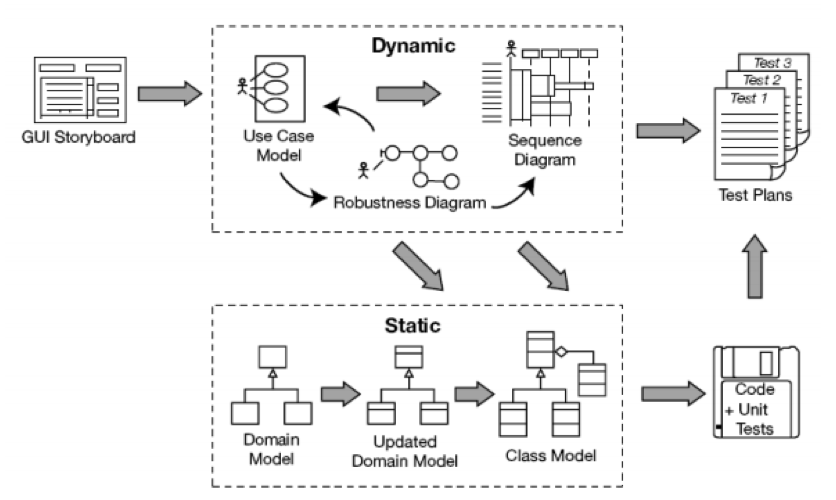
\includegraphics[scale=0.95]{./imagens/visao_geral_iconix.png}}
	\caption[Uma visão geral do ICONIX e seus componentes.]
	{Uma visão geral do ICONIX e seus componentes. \textbf{Fonte:} \citeonline{rosenberg_scott_use_case_driven_object_modeling_with_uml}}
	\label{fig:exemplo1}
\end{figure}

\newpage %Pular pagina para que o texto fica abaixo da imagem na nova pagina


\par Por proporcionar esta praticidade, o ICONIX será empregado para o desenvolvimento deste projeto, pois por meio dele é possível obter produtividade no desenvolvimento do \textit{software} ao mesmo tempo em que alguns artefatos são gerados, unindo o aspecto de abrangência e agilidade.
